\chapter{Technical specifications}
\label{chap:tech}
SALSA onsala is a modified television antenna with a diameter of 2.3~m and designed
to operate at 1420\,MHz.

\section{Angular resolution and accuracy}
\label{sect:ares}
SALSA has an angular resolution of about 5.4$^\circ$ (\emph{full width half
maximum}) at 1420\,MHz. This value has been measured using the Sun, see Fig.
\ref{fig:beam}. For comparision, remember that the full moon has an angular
diameter of about half a degree, or 30~minutes of arc. The tracking is limited
by the mechanical design to an accuracy of about 0.5$^\circ$.  We are working
to make the telescope even more accurate by improving the hardware design. Note
that the accuracy is always the same for any position, any error present for
one observation does not carry or accumulate to the next one.  This means that
while the position may have a small error, the error will never get worse even
if you observe for a very long time. 
\begin{figure}[ht]
\begin{center}
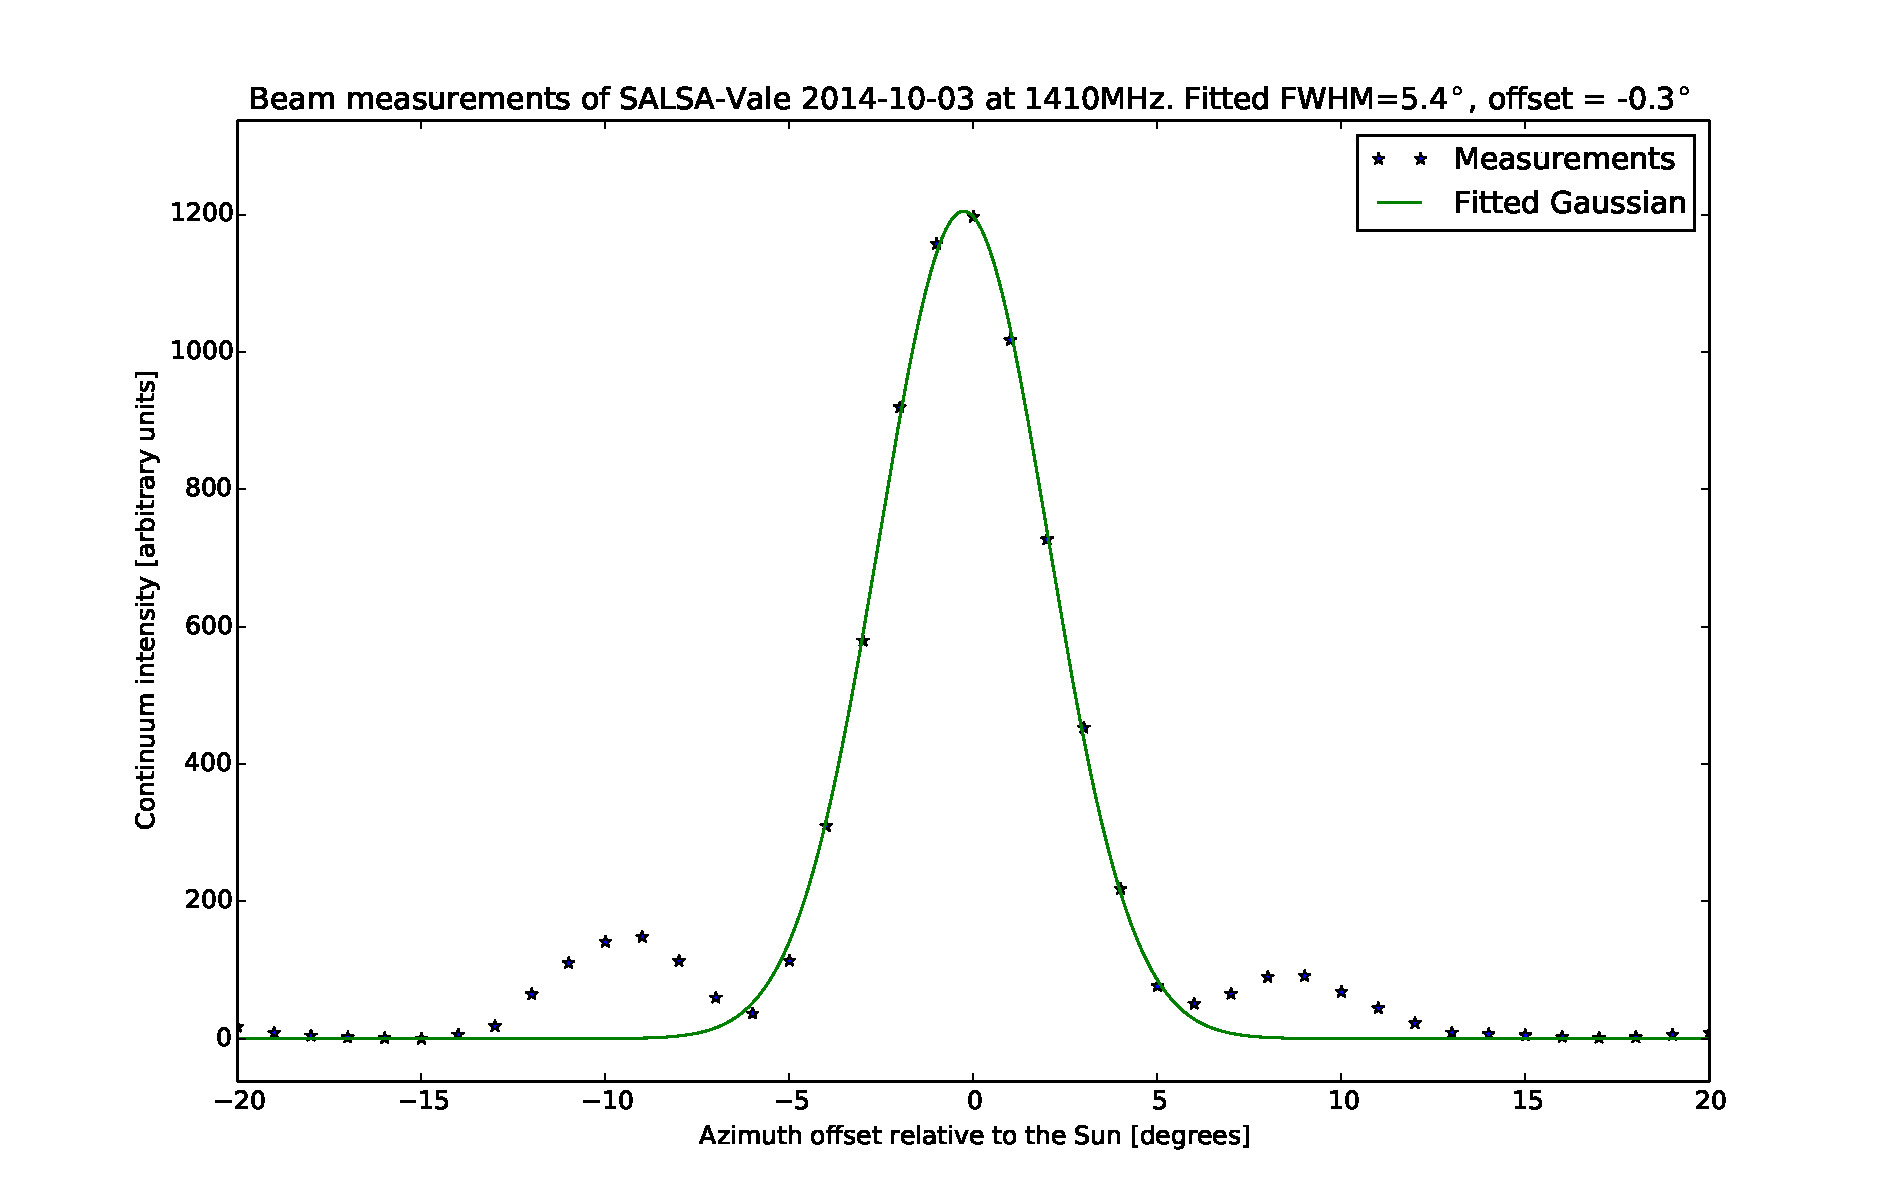
\includegraphics[width=\textwidth]{../figures/Beam_vale_2014-10-03.pdf}
\end{center}
\caption{The beam of Vale measured using the Sun at 1410\,MHz. A Gaussian fit
gives the FWHM=5.4$^\circ$. The sidelobes of the Sinc-function are clearly
visible, as expected for a circular aperture.}
\label{fig:beam}
\end{figure}

\section{Spectral resolution and accuracy}
The telescope uses the \emph{Universal Software Radio Peripheral} (USRP) to
record data. The USRP acts as a sampler which records a time stream to the hard
drive of the control computer. The channelisation, i.e. construction of the
spectrum, is done in software (FFT). This means that the number of channels
(spectral resolution) is not fixed, nor is the bandwidth. The spectral
resolution is limited by the free space and processing speed of the control
computer. Up to 10\,MHz bandwidth with 8192 channels have been tested, but for
most observations the standard settings of 2\,MHz bandwidth and 256 channels
are sufficient, i.e. a frequency resolution of 7.8\,kHz per channel. If a finer
resolution is needed, it may be selected from the \emph{Advanced} tab in the
\emph{Receiver control} part of the SALSA control program, but we cannot offer
support for these advanced modes yet.
